\section{Motivating example}
\label{sec:motivation}

\begin{enumerate}
\item Consider case where we want two charts showing two aggregations (Figure~\ref{fig:pipeline} above)
\item In Python, I load data, do some Pandas aggregation, build charts
\item This does not give me linking! We do not know how the charts relate!
\item I have to use Bokeh, but then I also have to rewrite how I aggregate (Figure~\ref{fig:pipeline} below)
\item Now I get some linking between two parts, but still not with the table that shows the data
\item Then you're also restricted in what you can do in your transformations
\item This is stupid, we should not have to do this. With our system, the programming language
  automatically provides the infrastructure that is necessary for linked brushing - in other words,
  everything runs on the same substrate.
\end{enumerate}

\begin{figure}
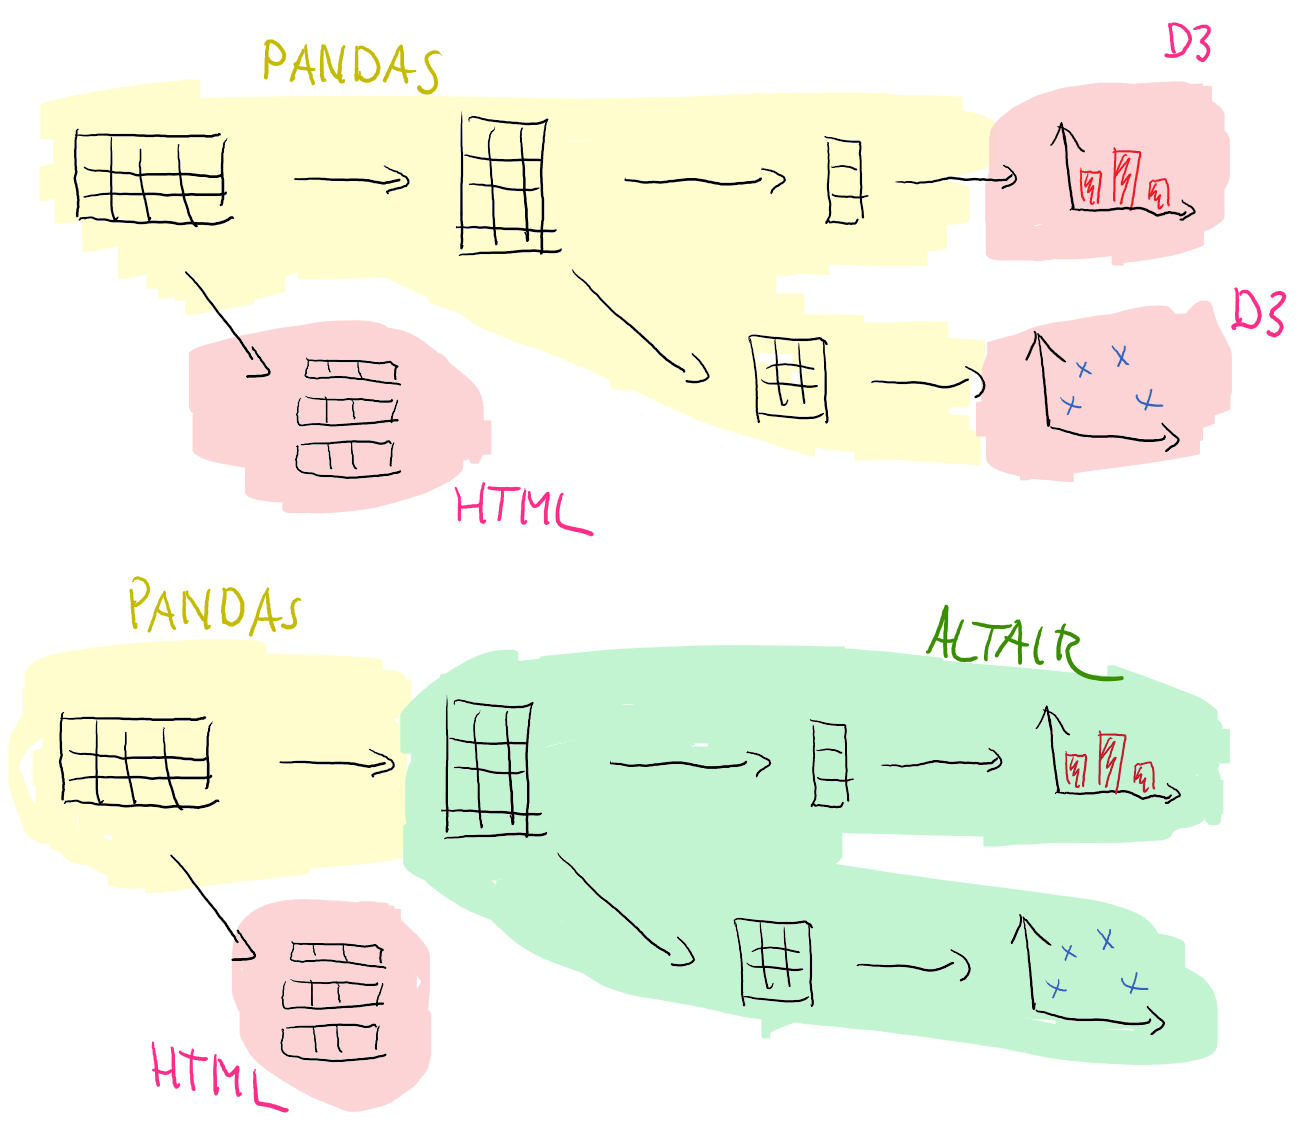
\includegraphics[scale=0.35]{image/pipeline}
\caption{Pipeline}
\label{fig:pipeline}
\end{figure}
